\chapter{ND280 software and existing ECal event reconstruction}
\label{chap:ND280Software}
The T2K experiment uses a bespoke software suite for simulation and analysis of ND280 data, which is based on the ROOT framework~\cite{Brun199781}.  The vast majority of the ND280 software suite utilises the oaEvent library which provides a unified framework for information manipulation and was specifically designed for this purpose.
As ND280 consists of many detector\Yoshi{}{ADDRESSED - check your apostrophes}s each providing a specific function, the ND280 software suite is designed to reflect this.  Not only are there specific software modules for individual subdetectors, there are specific modules for each phase of the subdetector information processing e.g. \Yoshi{Trip-T}{ADDRESSED - was trip-T. Be consistent with Chap 3} calibration, TPC reconstruction etc.  
\newline
\newline
As the software suite handles both production of simulated data and the processing of collected data, there are sections of the software chain which are specific to type of data being processed.  While the Monte Carlo simulation and real data do see different areas of the software chain, the general philosophy is to manipulate the Monte Carlo or the real data to a point where they can be treated as equals and them process them as such.  So, the description of the software will follow the same path: the Monte Carlo and real data specifics will be discussed first and then the unified treatment will follow. 
\section{Monte Carlo production software}
\label{sec:MCchain}
As described above, parts of the software chain are unique to simulated data processing.  Specifically, the simulation of the beam and the detector response need to be modelled before the Monte Carlo can be treated on equal footing with the real data.  This special processing is split into several steps, all of which are described below.

\subsection{Neutrino flux simulation}
\label{subsec:NeutrinoFluxSimulation}
The neutrino flux simulation uses Fluka2011~\cite{Ferrari_fluka:a} and a software set called JNUBEAM to model the J-PARC neutrino beam.  The process begins by using Fluka2011 to simulate the 30 GeV protons incident on the graphite target and their subsequent secondary interactions which produce the neutrinos parent mesons.  The kinematic information of the hadrons is then passed to the JNUBEAM simulation.  JNUBEAM is based on GEANT3~\cite{Brun:1987ma} and models the J-PARC secondary beamline.  The hadrons are tracked through the decay volume and are allowed to interact or decay to produce the simulated neutrino beam.  Importantly, all information associated with the daughter neutrinos and their parents are saved at this point.  By storing this information, the neutrino flux can be readily re-weighted to include new information associated with beam profile measurements or external data.
\newline
\newline
The main external tuning source is NA61/SHINE which is a hadron interaction experiment that uses a 31 GeV/c proton beam colliding with changeable targets~\cite{PhysRevC.84.034604}.  For use in the T2K flux simulation, NA61/SHINE has collected data using two graphite targets: one with a 4$\%$ nuclear interaction length thickness and a full T2K replica target.  The flux simulation used for this analysis is tuned using full replica target data.  Observed differences between the Fluka2011 simulation and NA61/SHINE data are used to re-weight the simulated neutrino flux.
\newline
\newline
Additionally to the external data, tuning measurements of the T2K beam profile are also used to re-weight the flux.  By making such measurements on a run-by-run basis, the simulated flux can be re-weighted to better model variations of the neutrino beam in each data run.
\subsection{Neutrino interaction simulation}
\label{subsec:NeutrinoInteractionSimulation}
After the neutrino flux has been modelled, simulation of the neutrino interactions with the T2K detectors follows.  The NEUT~\cite{Hayato2002171} event generator is used to simulate interactions with ND280.  The inputs to the interaction simulation are a neutrino vector file produced by the beam simulation and a ROOT based ND280 geometry.  The used geometry includes the magnetic field return yoke and everything contained within.  Using the inputs, NEUT tracks the neutrino and calculates the probability of interaction for every material it crosses.  To calculate the interaction probability, the potential interaction nucleus must be modelled.  For this, NEUT uses two models; the Moniz-Smith Relativistic Fermi Gas (RFG)~\cite{Miller2002223} and the O. Benhar spectral function models~\cite{Benhar1994493}.  The spectral functions are only implemented for carbon, oxygen and iron so the model used depends on the atomic number of the interaction candidate nucleus.  It is important to note at this point that this thesis deals with neutrino interactions on lead, so it is the RFG model that is used for signal interactions.
\newline 
\newline
The main interactions modes at T2K energies are quasi-elastic scattering (CCQE), single pion production  (CC1$\pi$) and Deep Inelastic Scattering (DIS) all of which have models in NEUT~\cite{LlewellynSmith1972261,Rein198179,1126-6708-2006-05-026}.
\newline
\newline
After the initial interactions, the final step is to simulate the final state interactions within the nucleus.  Each particle involved in the interaction is pushed through the nucleus in discreet steps with the probability of a final state interaction being calculated at each step.  If an interaction occurs, the final states of that interaction are also included in the subsequent steps.  This interactive procedure models the particle cascade until all the final states have reached the nucleus boundary.  At this point, all final state particles are recorded along with all of the information that created those particles.  This information is stored in a vector file and passed on to the ND280 detector MC package which handles the detector's response to these final state particles.
\subsection{ND280 detector simulation}
\label{subsec:ND280DetectorSimulation}
The simulation of the final state particles in ND280 is handled by nd280mc which is based on GEANT4~\cite{Agostinelli2003250} and ROOT.  The neutrino interaction vector files are taken as input and used as seeds in the detector simulation.  The neutrino vector inputs are not organised according to the J-PARC beam bunch structure so the detector simulation first groups the interactions into spills.  The beam intensity to be simulated is used to define how many interactions occur in a spill with Poisson fluctuations applied to that number.  The timing of the beam bunch structure is then used to group the interactions into bunches. 
\newline
\newline
nd280mc constructs a ROOT geometry of ND280 based on the design specifications of its subdetectors and then propagates the particles given to it by the neutrino generator through the geometry, simulating energy deposition, scattering and particle decay during propagation.

\subsection{Detector response simulation}
\label{subsec:DetectorResponseSimulation}
The next and final stage of the MC-only software chain is to model how the detector responds to the simulated particles propagating through it.  The detector response software, named elecSim, takes the output of nd280mc and models how the active regions of the detector would respond given an energy deposition in that region of the detector.  In the case of the calorimeters, elecSim handles the production of light produced by the constituent scintillator bars, how the light is propagated along the wavelength-shifting fibres and how the MPPCs would respond to the incident photons.  For the TPCs, the drift of the ionisation electrons through the gas and the subsequent response of the MicroMEGAS which receive them.  In all cases, the readout electronics response is simulated to produce a data-like output format.  This step concludes the section of the software chain which is specific to the MC.

\section{Real data processing software}
\label{sec:datachain}
The real data specific section of the software chain is very short.  Physics events deemed worth saving by any of the ND280 triggers are recorded by the detector and then saved for processing.  The MIDAS file format is used for storing the saved ND280 events.  All of the relevant information needed to process the event is stored in the MIDAS file, so the only unique step to the data processing is the conversion of the MIDAS file to the oaEvent format.  After the step, the oaEvent data files are exposed to the same software as MC files outputted by elecSim (see section~\ref{subsec:DetectorResponseSimulation}).


\section{Main software chain}
\label{sec:mainchain}
The aim of the rest of the software chain is to process the readout from the detector, be it simulated or collected data, and process it so essential information about the physics of the event can be extracted.  This is separated into three steps: calibration, reconstruction and data reduction/summarising.


\subsection{Detector calibration}
\label{subsec:DetectorCalibration}
The software package responsible for overseeing all aspects of the calibration stage is called oaCalib.  This controlling package passes the digitised signal from ND280 to dedicated calibration packages for the various kinds of readout electronics.  All of the information which can be extracted from an ECal event relies on the charge read by the MPPCs.  Thus, for the Trip-T detectors, like the ECals, the main aim of the calibration is to remove all electronic effects so that an accurate estimation of the charge read by the MPPCs can be made.  
\newline
\newline
Firstly, every MPPC is held at a bias in the absence of any signal to remove the non-linear dependence of the detector response on the lowest ADC channels.  This zero signal output is called the pedestal and must be subtracted from the charge readout by the MPPC.  
\newline
\newline
To estimate the number of photo-electrons produced in an MPPC, The readout charge is divided by the MPPC gain.  The breakdown voltage of an MPPC linearly varies with temperature (approximately 50 mV/$^\circ$C).  This translates to a percent level variation in the MPPC gain per degree.  This means small variations in temperature can cause a significant variation in the MPPC gain.  So, the gains for each channel are calculated and stored individually.
\newline
\newline
The time of the signal read by the MPPC is charge dependent and so it relies on the above corrections.  However, there are extra steps needed to get an accurate estimate of the timestamp.  The MPPC signal is given a timestamp once the charging capacitor exceeds a threshold value.  The time it takes to reach this threshold depends on the final collected charge of the MPPC.  This means that a lower charge signal would receive a later timestamp than a higher charge signal even if the signals occurred at the same time.  This effect is known as the electronic timewalk and is corrected for.
\newline
\newline
The light emission rate of the WLS fibres follows an exponential decay function which means that the emission rate depends on the total number of photo-electrons.  As described above, the Trip-T electronics only assign a timestamp once the collected charge passes a threshold.  So, the fibre decay causes a separate timewalk effect, called the fibre timewalk effect which is also corrected for.  
\subsection{Event reconstruction}
\label{subsec:EventReconstruction}
Once the information has been calibrated it is passed to the ND280 reconstruction software.  The reconstruction algorithms are separated into two phases: the local reconstruction and the global reconstruction.  The local reconstruction, which is run first, is separated into a set of algorithms specific to each subdetector.  Each subdetector reconstruction attempts to form its own picture of the event which passed through it.  After this, all of the local reconstruction information is passed to the global reconstruction which attempt to match and refit the subdetector results to maximise the amount of extractable information.

\subsection{Data reduction and summarising}
\label{subsec:DataReduction}
The final stage of the processing chain is to reduce and summarise all of the previous steps in the chain such that they are in a suitable format for the analyser.  A lot of the information, particularly from the reconstruction stage, is stripped out and the physics related objects are extracted.  Most importantly, all of the information is summarised in a pure ROOT format, meaning the analyser does not rely on the oaEvent library to analyse ND280 data.


\section{ECal event reconstruction}
\label{sec:ECalEventReconstruction}
As mentioned in section~\ref{subsec:EventReconstruction}, part of the reconstruction process is to run algorithms specific to the ND280 subdetectors.  The ECal is no exception and is equipped with an extensive suite of reconstruction algorithms designed to reconstruct events originating from the tracker region of ND280.  The inputs to the reconstruction are the calibrated scintillators bar hits which are used to form 3D objects and attach a topology hypothesis.

\subsection{Hit preparation}
\label{subsec:ECalHitPerparation}
The initial ECal reconstruction stage takes the hits outputted by the calibration stage and prepares them for the downstream algorithms.  The ECal hits arrive with timestamps but are not separated according to the bunch structure.  So, the hits are ordered in time and then grouped into buckets where a new bucket starts when a greater than 50~ns gap appears between two time-adjacent hits.  A second filter is then applied to arrange the hits according to the sensor they occurred on.  For double ended bars with both sensors activated, the time of the hit is re-estimated by averaging the timestamp of the two sensors.  The two hits are then merged to form a single hit.
\newline
It is then necessary to apply extra calibrations to the charges of the hits.  The effect of light attenuation along the WLS fibre is corrected for and a scaling is applied to convert the charge into MIP equivalent units (MEU).

\subsection{Basic clustering}
\label{subsec:ECalBasicClustering}
The time ordered hits are then passed to a set of clustering algorithms which attempts to form an object out of the ECal hits.  The first stage of this is called basic clustering which is a nearest neighbour algorithm designed to form 2D clusters of hits for both views of an ECal module.  This is initiated by forming a 30 ns window and searching for the highest charge hit contained within it to form a seed.  The seed cluster is expanded by searching for and adding candidate hits which pass the following criteria:
\begin{itemize}
  \item Is located in the 30 ns time window
  \item Is at most one bar away from a hit in the cluster
  \item Is at most two layers away from a hit in the cluster
\end{itemize}
To qualify as a basic cluster, any formed candidate must contain at least three hits.  The successfully formed clusters in both views of the ECal modules are then passed to the next stage of the clustering algorithms. 

\subsection{Cluster combination}
\label{subsec:ECalCombineClusters}
The second stage of the clustering algorithm takes the basic clusters in a given view and attempts to form merged clusters if a set of conditions are passed.  The cluster with the highest number of hits is taken as a seed and compared with all other clusters in the same view.  A Principal Components Analysis (PCA) is applied to all 2D clusters as the primary axis is used in one of the merging criteria.  A candidate cluster is merged with the seed cluster if:
\begin{itemize}
  \item The distance of closest approach, taken from the primary axes, of the candidate and seed cluster is less than 80~mm
  \item The charge weighted average hit times of the candidate cluster is within 40 ns of the seed cluster
  \item The charge weighted average distance of the candidate cluster to the seed cluster is less than 400~mm
\end{itemize}
All candidate clusters which pass the conditions are merged with the seed cluster.  After all comparisons have been made, a new seed cluster is found and the process is repeated until no more merges take place.  All clusters in each ECal view are then passed into the next clustering algorithm.



\subsection{Cluster expansion}
\label{subsec:ECalExpandClusters}
The next and final stage of the 2D clustering attempts to merge any unmatched hits with the already formed clusters if the comparison passes a set of conditions.  As before, a PCA is applied to all 2D clusters to calculate the primary and secondary axes as, again,  these are used in one of the matching conditions.  Let $\vec{n}_{\mathrm{pri}}$ and $\vec{n}_{\mathrm{sec}}$ be the primary and secondary axes of a cluster found by the PCA.  The squared spread of the cluster along the primary or secondary axis is then defined as
\begin{equation}
  \sigma_A^2 = \sum_{\alpha = x,y,z} \sigma_\alpha^2n_{A,\alpha}^2,
\end{equation}
where $A$ refers to either the primary or secondary axis and $\sigma_\alpha$ refers to the cluster's spread along the Cartesian axes.  A metric for defining how well the hit matches to the cluster can then be defined as 
\begin{equation}
  w = \sqrt{\Bigg(\frac{\vec{H}\cdot \vec{n}_{\mathrm{pri}}}{\sigma_{\mathrm{pri}}}\Bigg)^2 +  \Bigg(\frac{\vec{H}\cdot \vec{n}_{\mathrm{sec}}}{\sigma_{\mathrm{sec}}}\Bigg)^2},
\end{equation}
where $H$ is the vector joining the charge-weighted centre of the cluster and the centre of the hit.  The unmatched hit is merged with the 2D cluster if:
\begin{itemize}
  \item The unmatched hit is within 6 ns of one of the constituent hits of the 2D cluster
  \item The difference in bar number of the unmatched hit and at least one of the constituents hits in the 2D cluster is less than 11
  \item The difference in layer number of the unmatched hit and at least one of the constituents hits in the 2D cluster is less than 21
  \item The calculated value of $w$ is less than 50
\end{itemize}
Unlike the previous stage where it is possible to merge every cluster in a view, an unmatched hit can be matched with one, and only one, 2D cluster. So, not only does the hit-cluster comparison have to pass the relevant criteria, the comparison has to be a better match than all other comparisons.  In cases where the unmatched hit passes all of the conditions with more than one cluster, the comparison which provides the lowest $w$ is selected as the best match.
\newline
\newline
The 2D clusters in each view are then passed on to the final stage of the clustering algorithms.

\subsection{3D cluster formation}
\label{subsec:ECal3DMatching}
The final stage of the clustering algorithm attempts to form full 3D clusters using information from both view of an ECal module.  To do this, the algorithm takes the 2D clusters from one view and matches them with the 2D clusters in the other view.  All 2D clusters from one view are compared to all 2D clusters in the other view and the two that are the best match form a 3D cluster.  The metric used for the matching is a simple likelihood based on three input variables.  The first variable is the ratio of the total charge of the 2D matching candidate clusters, $Q_{\textrm{ratio}}$.  Assuming the two 2D clusters come from the same particle, the amount of charge deposited in each view should be similar, so $Q_{\textrm{ratio}}$ should be \sim1.  The $Q_{\textrm{ratio}}$ value is then compared with a probability density function generated using ND280 MC to retrieve $\mathcal{L}_{Q_{\textrm{ratio}}}$.  The second input variable to the likelihood compares the first layer used by the two matching candidate clusters which is closest to the ND280 tracker region, $\Delta_{\textrm{layer, first}}$.  If the two candidate clusters are created from the same particle, the difference in starting layer number should ideally be one.  As with with $Q_{\textrm{ratio}}$, the $\Delta_{\textrm{layer, first}}$ found for the matching candidates is compared to a probability density function to retrieve $\mathcal{L}_{\Delta_{\textrm{layer, first}}}$.  The final input to the likelihood is almost identical to the second input.  The variable, called $\Delta_{\textrm{layer, last}}$ compares the difference in layer number furthest away from the ND280 tracker region.  Besides this difference, $\Delta_{\textrm{layer, last}}$ is treated in exactly the same manner as $\Delta_{\textrm{layer, first}}$ and so will not be described in any more detail.
\newline
Once the three inputs for the matching candidates have been calculated, the value of the matching likelihood is then
\begin{equation}
  \mathcal{L} = \mathcal{L}_{Q_{\textrm{ratio}}} \times \mathcal{L}_{\Delta_{\textrm{layer, first}}} \times \mathcal{L}_{\Delta_{\textrm{layer, last}}}.
\end{equation}
As mentioned above, all 2D clusters in one view are compared with all 2D clusters in the other view.  The matching pair which produce the highest value of $\mathcal{L}$ are counted as a match.  The matched pair are then removed from the pool and the process is repeated until no more matches can be made or the value of $\mathcal{L}$ falls below $e^{-5}$.  All matched clusters are now counted as 3D objects and are passed on to the rest of the ECal reconstruction algorithms.

\subsection{3D hit reconstruction}
\label{subsec:ECal3DHitReconstruction}
So far in the ECal reconstruction, it has only been possible to reconstruct 2/3 of the hit coordinates.  However, now that full 3D clusters have been formed, the information from both ECal views can be used to estimate the third hit coordinate which is the coordinate along the length of the bar.
\newline
\newline
The hits are separated into their respective 2D view and then the charge-weighted average position of each layer is calculated.  Then, to calculate the final hit coordinate, the nearest four layers from the other view are found and a linear least-squares fit is applied to their 2D coordinates.  The line found is then extrapolated into the layer of interest which provides the unknown hit coordinate.

\subsection{Energy reconstruction}
\label{subsec:ECalEnergyReconstruction}
The ECal was designed to catch electromagnetic particles originating from the tracker region of ND280, particularly photons from $\pi^0$ decays.  An integral part of particle shower reconstruction is estimation of the total energy of the incoming particle.  So, the next phase of the reconstruction is particle energy estimation under the assumption that the incident particle created a full contained particle shower upon entering the ECal module.  The range of the energy fitter is 25 MeV to 20 GeV which almost fully covers the range of energies seen in the ND280 ECals.  The energy fitter works by minimising a likelihood function which takes the total charge, charge RMS and charge skew of the 3D cluster as inputs.  For each of the three input variables, splines were generated using simple photon particle gun MC which relates the input variables to the true particle energy.  The minimizer generates an estimate of the true energy and, via the splines, retrieves the expected values of the input variables.  By minimising the distance between the measured input variables and those taken from the splines an accurate estimate of the particle energy is found.  This energy estimate, along with the 3D cluster itself, is then passed on to the final section of the ECal reconstruction.

\subsection{Event classification}
\label{subsec:ECalParticleIdentification}
The final section of the ECal reconstruction is to attach a topology hypothesis to the 3D cluster.  The routines currently separate the clusters into two categories: those that are shower-like and those that are track-like using an Artificial Neural Network (ANN).  This multi-variate analysis object takes multiple pieces of information about the 3D cluster which attempts to measure the energy deposition and shape of the cluster and returns a single number.  The value of the returned number suggests whether the reconstructed object is track-like or shower-like. The discriminator was tested using ND280 electron and muon control samples, the results of which are shown for the DS ECal in Fig.~\ref{fig:ECalTrShVal}.

\begin{figure}
  \centering
  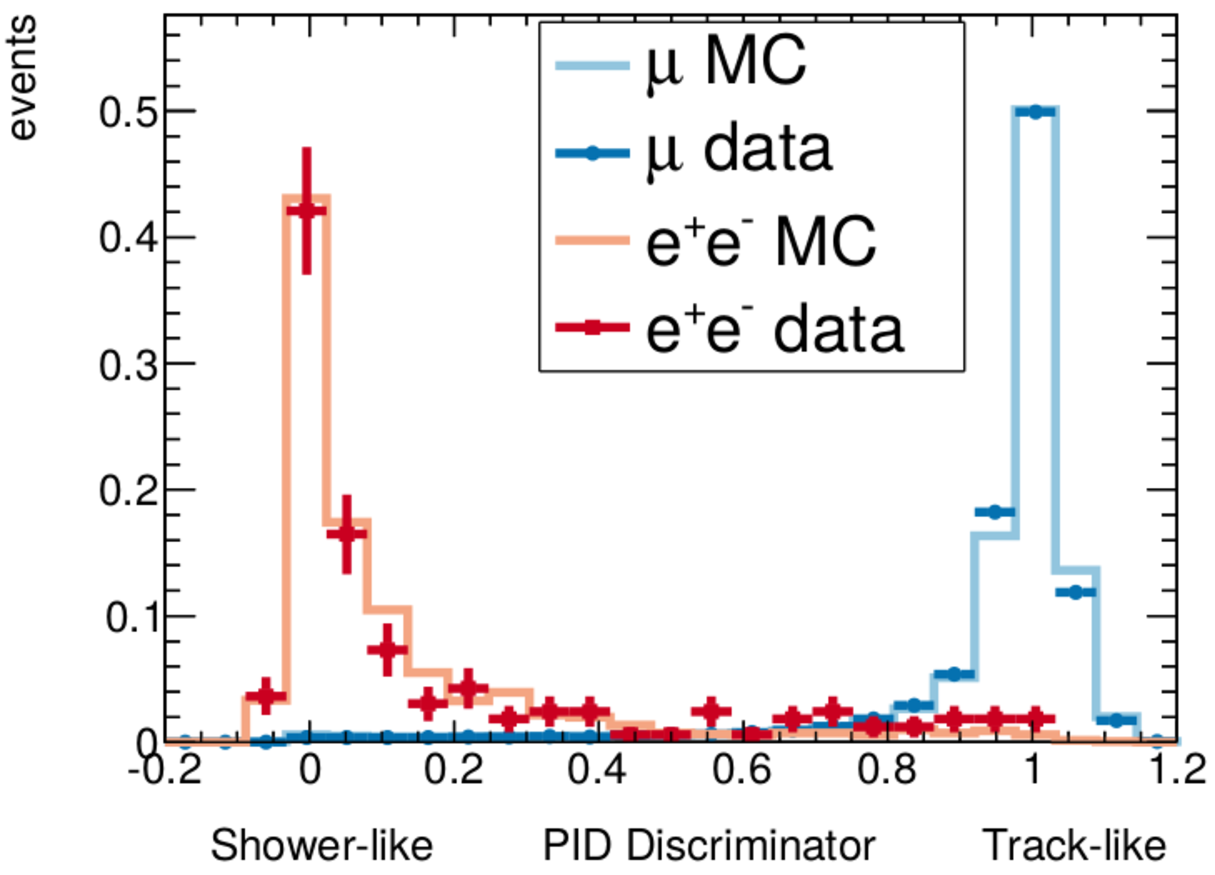
\includegraphics[width=11cm]{images/software/ecal_trshval.pdf}
  \caption{The track-like/shower-like discriminator for the DS ECal which is uses an Artificial Neural Network~(ANN)~\cite{1748-0221-8-10-P10019}.  Solid lines show the control sample Monte Carlo (based on NEUT simulation of beam events) and the points show the control sample data (taken from collected beam data).  For the muon samples, exactly one track is required in each of the TPCs and the DS ECal with an additional requirement that the TPC tracks are muon-like.  For the electron samples, photon pair production is checked in the FGD, requiring tracks with opposite charge with at least one TPC track which must be electron-like.  The muon and electron simulated distributions show good agreement with the collected data.\Yoshi{}{ADDRESSED - Say which reconstruction this comes from, and what the data and MC represent. The original caption carries way too little info}}
  \label{fig:ECalTrShVal}
\end{figure}


